\chapter{Обзор системы VLC}

\section{Li-Fi и VLC}

\Abbrev{IM}{intensity modulation}
\Abbrev{DD}{direct detection}
\Abbrev{IEEE (Institute of Electrical and Electronics Engineers)}{институт электроники и инжинеров электроники}

В VLC данные передаются при помощи модуляции интенсивности излучения источника (светодиода) \--- IM. Приёмником в такой системе может выступать фотодетектор, который использует принцип прямого детектирования (DD). VLC был придуман для связи <<от точки к точке>>, то есть как замена кабелям~\cite{Haas16}. Работа VLC описывается стандартом IEEE 802.15.7-2018~\cite{IEEE2018}.

С другой стороны, Li-Fi описывает полную беспроводную сеть с возможностью двусторонней коммуникации <<от точки к многим точкам>> и  <<от многих точек к точке>>. Помимо этого, Li-Fi включает в себя возможность использования многих точек доступа с быстрым переключением между ними, что позволяет обеспечить мобильность пользователей. То есть стандарт Li-Fi включает в себя стандарт VLC, что показано на схеме \ref{fig:vlcvslifi}.

\begin{figure}[!ht]
    \centering
    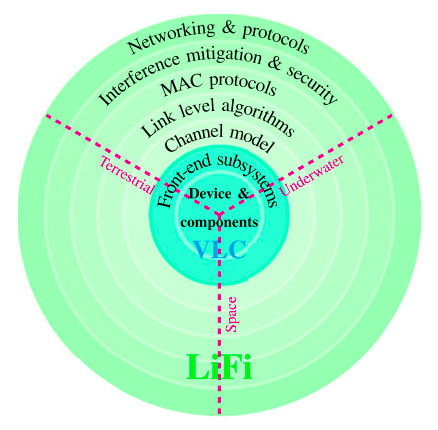
\includegraphics[width=.6\textwidth]{inc/img/vlcvslifi.png}
    \caption{Принципиальная схема Li-Fi и VLC~\cite{Haas16}}
    \label{fig:vlcvslifi}
\end{figure}

Как и было описано во введении, Li-Fi имеет ряд преимуществ по сравнению с Wi-Fi: он позволяет обеспечить безопасность передачи данных, отсутствие интерференции с ЭМ-приборами, разгрузка РЧ-спектра.

\section{Li-Fi передатчик}

Зачастую в системах передачи информации с помощью видимого света в качестве передатчика выбирается светодиодный светильник (LED luminaire)~\cite{LeMinh2008,Komine2006,Komine2004}. Он представляет из себя полноценное осветительное устройство, состоящее из LED источник излучения, балласта, корпуса и других компонентов. LED источник может состоять из одного или нескольких светодиодов, которые управляются с помощью управляющей микросхемы \--- контроллера, который контролирует ток, питающий светодиод и меняющий его яркость. Когда светодиодный светильник используется для коммуникации, контроллер модернизируется для передачи данных с помощью модуляции излучения. Примером простейшей модуляции является On-Off Keying, то есть <<нули>> и <<единицы>> передаются как два разных уровня интенсивности света.

Ключевым требованием к конструкции системы Li-Fi является то, что освещение, которое является основной целью светодиодных светильников, не должно нарушаться из-за использования связи. Таким образом, на работу Li-Fi системы влияет конструкция светодиодного светильника. Белый свет является самым используемым для освещения в помещениях и на улице. Это связано с тем, что цвет предметов под белым светом наиболее сильно похож на цвет предметов под естественным светом. Белый свет у LED светильников достигается двумя разными способами: 

\begin{enumerate}
    \item Синий LED с фосфором \--- этот источник генерирует белый свет с использованием синего LED, который покрыт жёлтым фосфором. Когда синий свет проходит через жёлтое покрытие, эта комбинация создаёт белый свет. При изменении толщины покрытия можно получать белый свет различной цветовой температуры.
    \item Комбинация RGB светодиодов \--- белый свет может быть получен при смешении красного, зелёного и синего света. Для этого, соответственно, необходимо три светодиода, что повышает стоимость светильника, по сравнению с синим фосфорным LED. 
\end{enumerate}

В осветительных системах чаще всего используется первый тип светодиодов из-за их дешевизны, однако в коммуникационных системах фосфорное покрытие значительно ограничивает скорость, с которой светодиод можно переключать, до нескольких МГц~\cite{Khalid2012}. С другой стороны, использование нескольких цветных светодиодов позволяет использовать Color Shift Keying модуляцию при помощи трёх длин волн, что позволяет получить высокую скорость передачи данных и низкую стоимость LED~\cite{Bian2019}.

\section{Li-Fi приёмник}

В качестве приёмников в Li-Fi системах чаще всего используются

\begin{enumerate}
    \item фотодетекторы \--- фотодиоды,
    \item датчики изображения \--- камеры.
\end{enumerate}

Фотодетектор \--- полупроводниковое устройство, которое генерирует ток при падении на него света. Современные коммерческие фотодетекторы могут детектировать с частотой до десятков МГц. 

\Abbrev{FPS (frames per second)}{кадры в секунду}
\Abbrev{IoT (internet of thing)}{интернет вещей}

Помимо него, возможно и использование камеры, так как они уже встроены в большинство потребительской техники (смартфоны, ноутбуки), что позволяет сделать эти устройства приёмниками в Li-Fi системе. Помимо этого, открывается возможность использования Li-Fi для интернета вещей (IoT)~\cite{Duquel2018}. По сути, камера является матрицей фотодетекторов на плате. Существенным недостатком является то, что так как камеры приспособлены для получения изображений высокого разрешения, используется большое количество фотодетекторов, что значительно снижает количество кадров в секунду (FPS) \--- скорость обработки излучения. Например, камеры современного смартфона позволяют записывать видео с 60 FPS, что означает, что использование камеры значительно ограничивает скорость получения информации. 

Важно отметить, что несмотря на то, что использование камеры позволяет превратить любое мобильное устройство в приёмник, пропускная способность остаётся очень ограничена (порядка килобит в секунду). В то же время отдельные фотодетекторы позволяют принимать информацию с высокой пропускной способностью (сотни мегабит в секунду).

\section{Методы модулирования излучения}

% http://www.phpathak.com/files/vlc-comsoccst.pdf p 10

Самое важное отличие системы связи по видимому свету от РЧ-связи заключается в том, что в VLC информация не может быть закодирована в амплитуде и фазе света~\cite{Tsonev2013}. Это означает, что техники модуляции, использующие модулирование фазы и амплитуды не могут быть применены в VLC, и информация должна быть закодирована в интенсивности света \--- модуляция интенсивности (IM). При создании Li-Fi системы необходимо учитывать параметры освещения, некоторые из которых могут повлиять на человека. Пример таких параметров: 
% Существуют различные техники модуляции интенсивности, некоторые из них будут рассмотрены ниже.

\begin{enumerate}
    \item затемнение (dimming). В~\cite{Zukauskas2002} было показано, что для разных действий необходимы разные уровни яркости освещения. Например, освещение в интервале $30-100$ лк обычно является достаточным для освещения общественных мест. С другой стороны, для освещения офисов и домов необходима освещённость порядка $300-1000$ лк. 
\item 
\end{enumerate}


% It was suggested in [17] that different levels
% of illuminance is required when performing different types
% of activities. As an example, an illuminance in the range of
% 30–100 lux is often enough for simple visual tasks performed
% in most public places. On the other hand, office or residential applications require higher level of illuminance in the
% range of 300–1000 lux. With the advancements in LED driver
% circuits, it has become possible to dim an LED to an arbitrary level depending on the application requirement to save
% energy.
% If an LED can be dimmed to an arbitrary level, it is also
% necessary to understand its impact on the human perceived
% light. It was first shown in [33] that the relation between
% the measured light and the perceived light is non-linear. This
% property is shown in Fig. 12. In other words, a human eye adapts
% to lower illumination by enlarging the pupil to allow more light
% to enter the eye. The perceived light can be calculated [33] from
% the measured light as